\newcommand\Model{\mathcal{M}}
\newcommand\eqnref[1]{\eqref{eq:#1}}
\newcommand\Hcf{H_{c \rightarrow f}}
\newcommand\Hcfhat{\hat{H}_{c \rightarrow f}}

\begin{abstract}
A number of recent papers have investigated the Manhattan world
assumption, in which surfaces in the world are assumed to be aligned
with one of three dominant directions
\cite{Coughlan99,Zhang02,Furukawa09,Lee09}. In this paper we present a
dynamic programming solution to the reconstruction problem for
``indoor'' Manhattan worlds (a sub--class of Manhattan worlds). Our
algorithm deterministically finds the global optimum and exhibits
computational complexity linear in both model complexity and image
size. This is an important improvement over previous methods that were
either approximate \cite{Furukawa09} or exponential in model
complexity \cite{Lee09}. We present results for a new dataset
containing several thousand manually annotated images, which are
released in conjunction with this paper.
\end{abstract}

\section{Introduction}

In this paper we investigate the problem of reconstructing geometric
models from single images. We choose to fit a model containing sparse
geometric primitives with the intended aim of higher--level
reasoning. If novel--view synthesis or photo-realistic 3D modelling
were the goal then a dense reconstruction may be appropriate, but if
the model is to be used as input to some reasoning problem, as is the
motivation for the present work, then a simpler model may be more
useful. In particular, when reasoning about indoor environments the
location of the floor, ceiling, and wall planes provide strong cues to
the probable locations of objects and events, whereas a raw point
cloud would be more difficult to interpret. Furthermore, simple models
have fewer degrees of freedom and are easier to infer from ambiguous
image evidence.

It is perhaps for this reason that the past few years have seen
considerable interest in the Manhattan world assumption
\cite{Coughlan99,Zhang02,Lee09,Furukawa09,Flint10}, in which each
surface is assumed to have one of three possible orientations. Making
this assumption introduces regularities that can improve the quality
of the final reconstruction \cite{Furukawa09}. Several papers have
investigated the even more constrained class of \textit{indoor}
Manhattan scenes \cite{Lee09,Flint10,Hedau09}, which consist entirely of
vertical walls extending between the floor and ceiling planes. A
surprisingly broad set of interesting environments can be modelled
exactly or approximately as indoor Manhattan scenes \cite{Flint10}. It
is with this class of scenes that this paper is concerned.

The present work describes a novel and highly efficient algorithm to
obtain models of indoor Manhattan scenes from single images using
dynamic programming. In contrast to point cloud reconstructions, our
algorithm assigns semantic labels such as ``floor'', ``wall'', or
``ceiling''. We show that our method produces superior results when
compared to previous approaches. Furthermore, our algorithm exhibits
running time linear in both image size and model complexity (number of
corners), whereas all previous methods that we are aware of
\cite{Lee09,Flint10} are exponential in model complexity.

The remainder of the paper is organised as follows. Section 2
describes previous work in this area and section 3 outlines our
approach. In section 4 we pose the indoor Manhattan problem formally,
then in section 5 we develop the dynamic programming solution. We
present experimental results in section 6, including a comparison with
previous methods. Concluding remarks are given in the final section.

\section{Background}

Many researchers have investigated the problem of recovering
polyhedral models from line drawings. Huffman \cite{Huffman71}
proposed a scheme to distinguish concave, convex, and occluding lines,
which allows discrimination between possible and impossible
objects. Waltz \cite{Waltz72} investigated a more general problem
involving incomplete line drawings and spurious measurements from
shadows. Sugihara \cite{Sugihara82} proposed an algebraic approach to
interpreting line drawings, while the ``origami world'' of Kanade
\cite{Kanade80} utilised heuristics to reconstruct a model of hollow
shells and planar sheets. These approaches were limited to synthetic
line drawings.

Hoiem \etal \cite{Hoiem05} and Saxena \etal \cite{Saxena09} have
investigated the single image reconstruction problem from a machine
learning perspective. Their approaches assign pixel--wise orientation
labels using appearance characteristics of outdoor scenes. Hedau \etal
\cite{Hedau09} extend this to indoor scenes, though their work is
limited to rectangular box environments.

The work most closely related to our own is that of Lee \etal
\cite{Lee09}, who have shown that line segments can be combined to
generate indoor Manhattan models using a branch--and--bound
algorithm. In contrast to their approach, our system uses dynamic
programming to efficiently search \textit{all} feasible indoor
Manhattan models rather than just those generated by line segments. As
a result we obtain more accurate models, can reconstruct more complex
environments (see \figref{positive-egs}), and obtain computation times
several orders of magnitude less than their approach, as will be
detailed in \sectref{results}.

Furukawa \etal \cite{Furukawa09} have used the Manhattan world
assumption for stereo reconstruction. Their models are of high
quality but their quoted computation times (of between one minute and
one hour forty minutes) make their approach unsuitable to on--line
applications. Their approach is not comparable to ours because they
use multiple calibrated views, and they search a different class of
models.

\section{Outline of Proposed Approach}

The Manhattan world assumption states that world surfaces are oriented
in one of three mutually orthogonal directions \cite{Coughlan99} and
the indoor Manhattan assumption further states that the environment
consists of a floor plane, a ceiling plane, and a set of walls
extending vertically between them \cite{Lee09}. Each wall therefore
has one of two possible orientations, and each corner is either
concave, convex, or occluding (see \figref{fin-egs}). Indoor Manhattan
models are interesting because they can represent many indoor
environments approximately or exactly, yet they introduce regularities
to the reconstruction problem that makes possible a left--to--right
decomposition of the scene, on which the dynamic programming algorithm
developed in this paper rests. Our approach to reconstructing indoor
Manhattan environments consists of the following five steps:
\begin{enumerate}
  \item{Identify dominant directions. (\sectref{vpts})}
  \item{Identify the floor and ceiling planes. (\sectref{fcmap})}
  \item{Warp the image to a canonical view. (\sectref{warp})}
  \item{Obtain weak orientation estimates. (\sectref{orient-est})}
  \item{Estimate the final model. (Sections 4 and 5)}
\end{enumerate}

\subsection{Identifying dominant directions}
\label{sect:vpts}

We identify three dominant directions by estimating mutually
orthogonal vanishing points in the image. We follow a similar approach
to Koseck\`{a} and Zhang \cite{Zhang02}, in which $k$--means
clustering is used to obtain an initial estimate, after which EM is
employed to identify the final vanishing points
$\vect{v_1}$,$\vect{v_3}$, and $\vect{v_3}$.

If intrinsic camera parameters are not provided then we construct the
camera matrix $K$ from the detected vanishing points by assuming that
the camera centre is at the image centre and choosing a focal length
and aspect ratio such that the calibrated vanishing points are
mutually orthogonal. For the remainder of this paper
$\vect{v_1}$,$\vect{v_2}$, and $\vect{v_3}$ denote the calibrated
vanishing points.

We assume that the vanishing point with largest absolute
$y$--coordinate represents the up--down direction in the world (\ie
the direction in which gravity operates), and by convention we always
label this direction $\vect{v_3}$. The horizon line is given by
$\vect{h}=\vect{v_1}\times\vect{v_2}$.

\subsection{Identifying the floor and ceiling planes.}
\label{sect:fcmap}

An indoor Manhattan scene has exactly one floor and one ceiling plane,
both with normal direction $\vect{v_3}$. It will be useful in the
following sections to have available the mapping $\Hcf$ between the
image locations of ceiling points and the image locations of the floor
points that are vertically below them (see \figref{fcmap}). $\Hcf$ is
a planar homology with axis $\vect{h}$ and vertex $\vect{v_3}$
\cite{Criminisi01} and can be recovered given the image location of any
pair of corresponding floor/ceiling points $(\vect{x_f},\vect{x_c})$
as
\begin{equation}
  \Hcf = I + \mu\frac{\vect{v_3}\vect{h}^T}{\vect{v_3} \cdot \vect{h}} ~,
\end{equation}
where $\mu = <\vect{v_3},\vect{x_c},\vect{x_f},
\vect{x_c}\times\vect{x_f}\times\vect{h}>$ is the characteristic cross
ratio of $\Hcf$.

\begin{figure}[tb]
\centering
\includegraphics[width=0.4\textwidth]{figures/fcmap}
\caption{The mapping $\Hcf$ transfers points between the ceiling and
  floor.}
\label{fig:fcmap}
\end{figure}

Although we do not have \textit{a priori} any such pair
$(\vect{x_f},\vect{x_c})$, we can recover $\Hcf$ using the following
RANSAC algorithm. First, we sample one point $\vect{\hat{x}_c}$ from
the region above the horizon in the Canny edge map, then we sample a
second point $\vect{\hat{x}_f}$ collinear with the first and
$\vect{v_3}$ from the region below the horizon. We compute the
hypothesis map $\Hcfhat$ as described above, which we then score by
the number of edge pixels that $\Hcfhat$ maps onto other edge pixels
(according to the Canny edge map). After repeating this for a fixed
number of iterations we return the hypothesis with greatest score.

Many images contain either no view of the floor or no view of the
ceiling. In such cases $\Hcf$ is unimportant since there are no
corresponding points in the image. If the best $\Hcf$ output from the
RANSAC process has a score below a threshold $k_t$ then we set $\mu$
to a large value that will transfer all pixels outside the image
bounds. $\Hcf$ will then have no impact on the estimated model.

\subsection{Warping the image to a canonical view}
\label{sect:warp}

The algorithms presented in the remainder of this paper will be
simplified if vertical lines in the world appear vertical
in the image. We therefore warp images according to a homography
\begin{equation}
  H = 
  \begin{pmatrix}
    \vect{v_3} \times \vect{e_3} \\
    \vect{v_3} \\
    \vect{v_3} \times \vect{e_3} \times \vect{v_3}
  \end{pmatrix}
  ~,
\end{equation}
where $\vect{e_3}=[0,0,1]^T$.

This step is not crucial to our approach and we could instead do all
geometric calculations in the original image. Hence, the fact that the
warped image will be contain a singularity if $\vect{v_3}$ is within
the image bounds does not restrict the applicability of our
approach. For the sake of simplicity, however, we present the
remainder of this paper assuming that $\vect{v_3}$ is outside the
image bounds.

\subsection{Obtaining weak orientation estimates}
\label{sect:orient-est}

Our algorithm requires a pixel--wise surface orientation estimate to
bootstrap the search. Obtaining such estimates has been explored by
several authors \cite{Lee09,Hoiem05,Saxena09}. We adopt the simple and
efficient line--sweep approach of Lee \etal \cite{Lee09}, which
assigns one of four labels $\{1,2,3,z\}$ to each pixel, where $z$
represents an unknown orientation and the remaining labels identify
the normal direction of the surface that generated the pixel. We
denote the orientation map $o:\mathbb{R}^2\rightarrow \{1,2,3,z\}$.

Note that our algorithm is is not dependent on the manner in which $o$
is obtained; any method capable of estimating surface orientations
from a single image, including the work of Hoiem \cite{Hoiem05} or
Saxena \cite{Saxena09}, could be used instead.

We generate four binary images $B_i$ such that pixel $B_i(\vect{x})=1$
if and only if $o(\vect{x})=i$. We then compute the integral image
\cite{Viola01} for each $B_i$, which allows us to count the number of
pixels of a given orientation within any rectangular sub--image in
$O(1)$ time. This represnetation expediates evaluation of the cost
function described in the following section.

\section{Problem statement}
\label{sect:probstmt}

We represent an indoor Manhattan model $\Model$ as an alternating
sequence of corners and walls $\{c_1,W_1,c_2,W_2,...,W_{n-1},c_n\}$,
$c_i < c_{i+1}$. Each corner $c_i$ is the column index at which two
walls meet, and each wall $W_i=(r_i,a_i)$ comprises an orientation
$a_i\in\{1,2\}$, which determines whether its vanishing point is
$\vect{v_1}$ or $\vect{v_2}$, and a row index $r_i$ at which its upper
edge meets the corner to its left. An example model is shown in
\figref{model-params}. Remarkably, this simple description completely
specifies all four corners of each wall segment (see
\figref{pqrs}). Clockwise from top--left the vertices of the i\th wall
are
\begin{eqnarray}
  \vect{p_i} &=& [c_i,r_i,1]^T \\
  \vect{q_i} &=& \vect{p_i} \times \vect{v_{a_i}} \times
       [1,0,-c_{i+1}]^T \\
  \vect{r_i} &=& H_{c \rightarrow f} \vect{q_i} \\
  \vect{s_i} &=& H_{c \rightarrow f} \vect{p_i} ~.
\end{eqnarray}

\begin{figure}[tb]%
  \centering
  \subfloat[][]{%
    \label{fig:pqrs}
    \includegraphics[width=0.6\textwidth]{figures/pqrs}}
  \subfloat[][]{%
    \label{fig:model-params}
    \includegraphics[width=0.4\textwidth]{figures/model-params}}
  \caption{(a) An illustration of the model
    $\Model=\{c_1,(r_1,a_1),...,(r_4,a_4),c_5\}$; (b) the values
    $(c_i,r_i,a_i,c_{i+1})$ fully specify the four corners of a wall.}
\end{figure}

A model $\Model$ predicts one of three possible surface orientations
$\mathcal{L}=\{1,2,3\}$ for each pixel $\vect{x}$. We denote this
prediction $\Model(\vect{x})\in\mathcal{L}$ where
\begin{equation}
  \Model(\vect{x}) =
  \begin{cases}
    a_i & \mbox{if } \vect{x} \in
    \mbox{quad}(\vect{p_i},\vect{q_i},\vect{r_i},\vect{s_i}) \\
    a_v & \mbox{otherwise}
  \end{cases}
  ~,
\end{equation}
where $a_v$ is the index of the vanishing point representing the
vertical direction in the world.

Not all models $\Model$ are physically realisable, but those that are
not are easily discarded using simple tests on the locations of walls
and vanishing points as enumerated by Lee \etal \cite{Lee09}. The
reader is referred to their paper for details; we simply note that a
model is feasible if all of its corners are feasible, and the
feasibility of a corner is dependent only on the immediately adjoining
walls.

We are now ready to state the minimisation problem formally. Given an
input image of size $W \times H$ and an orientation map $o$, we define
the cost of assigning pixel $\vect{x}$ label $l \in \mathcal{L}$ as
\begin{equation}
  C_p(\vect{x},l) =
  \begin{cases}
    0, & \mbox{if } o(\vect{x}) = l \mbox{ or } o(\vect{x}) = z \\
    1, & \mbox{otherwise}\\
  \end{cases}
  ~.
\end{equation}
The overall cost for a model $\Model$ containing $n$ corners is then
\begin{equation}
  \label{eq:cost}
  C(\Model) = \lambda n - \sum_{\vect{x}\in\mathcal{I}} C_p(\vect{x},\Model(\vect{x}))
\end{equation}
where $n\lambda$ is the regularisation term. We seek the model
$\Model^*$ with minimum cost
\begin{equation}
  \label{eq:opt-model}
  \Model^* = \underset{\Model}{\operatorname{argmax}} ~ C(\Model)
  ~.
\end{equation}

Finally, the marginal cost $C_w$ of the $i$\th wall $W_i=(r_i,a_i)$ is
\begin{equation}
  C_w = \sum_{x_i\leq x\leq x_{i+1}} \Bigl(
  \sum_{1 \leq y \leq U_i} C_p(x,y,a) +
  \sum_{U < y \leq L_i} C_p(x,y,a_v) +
  \sum_{L < y \leq H} C_p(x,y,a) \Bigr)
\end{equation}
where $L_i$ and $U_i$ are respectively the ceiling/wall and floor/wall
intersection at column $x_i$. The three sums over $y$ are $O(1)$
operations given the integral images described in
\sectref{orient-est}.

\section{Proposed algorithm}
In this section we present a dynamic programming solution to the
problem posed in \sectref{probstmt}. We develop the algorithm
incrementally to assist readability. Our solution rests on a
decomposition of the indoor Manhattan problem into a set of
sub--problems that can be solved in terms of one another. Consider the
following sub--problem.

Let $f_{in}(x,y,a,k)$ be the cost of a model $\Model^+ =
\{c_1,W_1,...,W_{n-1},c_n\}$ such that
\begin{enumerate}
  \item{$n=k$, (\ie $\Model^+$ contains $k$ corners),}
  \item{$c_n=x$ (\ie the rightmost corner is at column $x$),}
  \item{$W_{n-1}=(y,a)$
    (\ie wall $n-1$ terminates at row $y$ with orientation
    $a$),}
  \item{$\Model^+$ is feasible, and}
  \item{$\Model^+$ has minimal cost among all such models.}
\end{enumerate}

We show in the additional material that if a model
\begin{equation}
  \Model=\{c_1,W_1,...,W_{k-1},c_k\}
\end{equation}
is a solution to the sub--problem $f_{in}(c_k,r_k,a_k,k)$, then the the
truncated model
\begin{equation}
  \Model'=\{c_1,W_1,...,W_{k-2},c_{k-1}\}
\end{equation}
is a solution to the sub--problem $f_{in}(c_{k-1}, r_{k-1}, a_{k-1},
k-1)$.

In light of this fact we introduce the following recurrence relation:
\begin{equation}
  \label{eq:fin-recurrence-first}
  f_{in}(x,y,a,k) = \min_{x'<x,~y',a'} \Bigl( f_{in}(x',y',a',k) +
  C_w \Bigr) ~,
\end{equation}
where $C_w$ is the marginal cost of the wall $W=(y',a')$. We also
introduce the following boundary conditions:
\begin{equation}
  \label{eq:fin-base}
  f_{in}(x,y,a,k) =
  \begin{cases}
    0, & \mbox{if } x=0 \\
    \infty, & \mbox{if } k<0 \mbox{ and } x>0
  \end{cases}
  ~,
\end{equation}
which are justified, respectively, because a model with rightmost
corner at $x=0$ does not span any part of the image, so its cost must
be zero, and because a model cannot contain less than zero corners.

Finally, the cost of the optimal model \eqnref{opt-model} is
\begin{equation}
  \label{eq:opt-entry-point}
  C(\Model^*) = 
  \min_{{1\leq y \leq H \atop k \leq K} \atop a\in\{1,2\}}
  \Bigl( f_{in}(W,y,a,k) - \lambda k \Bigr) ~.
\end{equation}
where $K$ is a parameter specifying the maximum model complexity and
$\lambda$ is the per--wall penalty.

We compute $C(\Model^*)$ by recursively evaluating $f_{in}$
according to \eqnref{fin-recurrence-first} until we reach one of the
boundary conditions \eqnref{fin-base}. In line with the standard
dynamic programming approach we cache each evaluation to avoid
evaluating the same node multiple times. Once all nodes have been
evaluated, $\Model^*$ is obtained by back--tracking through the
evaluation graph.

\begin{figure}[tb]
\centering
\includegraphics[width=0.75\textwidth]{figures/fin-hypotheses}
\caption{Three models that satisfy constraints 1--4 for the
  sub--problem $f_{in}(x,y,a,k)$. There will only be one such model
  that satisfies the minimal cost constraint. Note that the
  right--most wall in each model terminates at $(x,y)$ with
  orientation $a$.}
\label{fig:fin-egs}
\end{figure}

\textbf{Complexity.} Since each node is evaluated at most once, the
overall complexity is given by the product of the number of nodes and
the complexity of evaluating each node. The latter is $O(W^2H)$, since
the minimisation in \eqnref{fin-recurrence-first} is over $O(WH)$
terms and computing the marginal cost $C_w$ requires $O(W)$
additions. The number of nodes is $O(WHK)$, so the overall complexity
of the basic algorithm is $O(W^3H^2K) = O(L^5K)$ where $L=\max(W,H)$.

\subsection{Auxiliary nodes}

The basic algorithm is hampered by the need to minimise simultaneously
over $x'$ and $y'$ in \eqnref{fin-recurrence-first}. In this section
we show how to decouple these minimisations by introducing auxiliary
sub--problems, which results in a significant reduction in
computational complexity.

We introduce three new sub--problems: $f_{up}$, $f_{down}$, and
$f_{out}$. Each of these is defined identically to $f_{in}$, except
that constraint 3 is replaced according to the following table:

\begin{tabular}{p{0.1\textwidth}p{0.75\textwidth}}
  $f_{up}$ & $r_{n-1} \leq y$ (\ie the rightmost wall terminates above
  row $y$) \\
  $f_{down}$ & $r_{n-1} \geq y$ (\ie the rightmost wall terminates 
  below row  $y$) \\
  $f_{out}$ & appending a wall $W=\{y,a\}$ to $M^+$ would result in a
  feasible model. \\
\end{tabular}

Using a similar argument to that given in the previous section it can
be shown that these sub--problems are related by the following
recurrence relations:
\begin{eqnarray}
  \label{eq:fout-recurrence}
    f_{out}(x,y,a,k) &=& \min_{a'\in\{1,2\}} \min
      \begin{cases}
        f_{up}(x,y,a',k) & \\
        f_{out}(x,y,a',k) & \\
        f_{down}(x,y,a',k) &
      \end{cases}
\end{eqnarray}
\begin{eqnarray}
  \label{eq:fup-recurrence}
  f_{up}(x,y,a,k) &=& 
  \begin{cases}
    \min \Bigl(f_{in}(\cdot), f_{up}(x,y-1,a,k)\Bigr), &
    \mbox{if } y \geq 1 \\
    \infty, & \mbox{otherwise}
  \end{cases}
\end{eqnarray}
\begin{eqnarray}
  \label{eq:fdown-recurrence}
  f_{down}(x,y,a,k) &=& 
  \begin{cases}
    \min \Bigl(f_{in}(\cdot), f_{down}(x,y+1,a,k)\Bigr), &
    \mbox{if } y \leq H \\
    \infty, & \mbox{otherwise}
  \end{cases}
\end{eqnarray}
\begin{eqnarray}
  \label{eq:fin-recurrence-basic}
  f_{in}(x,y,a,k) &=&
  \begin{cases}
    0, & \mbox{if } x=0 \\
    \infty, & \mbox{if } k<0 \\
    \min_{x'<x}\Bigl(f_{out}(x',v(x'),a,k-1)+c(x')\Bigr), &
    \mbox{otherwise}
  \end{cases}
\end{eqnarray}
where in the final equation $v(x')$ is the $y$--coordinate at which
the line through $\vect{v_a}$ and $(x,y)$ meets column
$x'$. Feasibility is enforced by removing either or both of the $f_{up}$
or $f_{down}$ terms in \eqnref{fout-recurrence} if such a corner would
result in an infeasible model.

\subsection{The line--jump optimisation}
Evaluating a $f_{in}$ node remains an $O(W)$ operation due to the
minimisation over $x'$ in \eqnref{fin-recurrence-basic}. In this
section we show how to reduce this to an $O(1)$ operation.

\begin{figure}[tb]
\centering
\includegraphics[width=0.4\textwidth]{figures/pixel-residuals}
\caption{A line from $\vect{x}$ to $\vect{v_a}$, and the distances $d$
  to nearby pixel centres (green dots). The starred pixel is the first
  that satisfies $d<\alpha$.}
\label{fig:pixel-residuals}
\end{figure}

Consider \figref{pixel-residuals}, showing a line from a pixel at
$\vect{x}$ to a vanishing point. If the line passed exactly through
some other pixel centre $\vect{x_p}$ then we could simply evaluate
$f_{in}(x_p,y_p,a,k)$ and terminate the line search at that point. It
is unlikely that the line will pass exactly through an integer--valued
pixel centre, so we instead specify a threshold $\alpha$ within which
a pixel centre will be considered to fall exactly on a line. We suffer
no loss of precision by doing this since the image itself is precise
only up to pixelation. We now have
\begin{equation}
  \label{eq:fin-recurrence}
  f_{in}(x,y,a,k) = \min
  \begin{cases}
    \min_{x_p \leq x' < x}\Bigl(f_{out}(x',v(x'),a,k-1)+c(x')\Bigr) & \\
    f_{in}(x_p,v(x_p),a,k-1)+c(x_p) & \\
  \end{cases}
  ~.
\end{equation}
where $(x_p,y_p)$ is the closest pixel to $(x,y)$ satisfying $x_p<x$
and for which $d=\vect{x} \cdot (\vect{x_p} \times \vect{v_a})$ is
less than $\alpha$. Both $(x,y)$ and $\vect{v_a}$ have integer
coordinates since they are observed at pixel locations, so we have the
upper bound
\begin{equation}
  x-x_p<\beta
\end{equation}
for some constant $\beta$, which is dependent only on our choice for
$\alpha$ \cite{Schrijver98}.

\textbf{Complexity.} Evaluating each node is now an $O(1)$
operation, so the overall complexity of our algorithm is given by the
number of nodes in the evaluation graph, which is
\begin{equation}
  O(KL^2) ~.
\end{equation}

\subsection{Down--sampling the orientation map}

As a further optimisation we down--sample the orientation map $o$,
replacing each $m \times m$ block of cells with a single cell
containing the majority vote over the block. This reduces both the
number of nodes in the graph and the cost of evaluating $C_w$.

\section{Other approaches}

\textbf{Graph cuts. }
\label{sect:comp-graph-cuts}
Many pixel--labelling problems have been successfully solved using
graph cuts. Kolmogorov and Zabih \cite{Kolmogorov02} have investigated
the class of cost functions that can be minimised using graph cuts.
Their work demonstrates that \textit{regularity}, a special case of
sub--modularity, is a necessary condition for any energy function to be
minimised via graph cuts.

It turns out that the cost \eqnref{cost} is not regular, so cannot be
minimised using graph cuts. Intuitively this is because the indoor
Manhattan constraint induces complicated dependencies between the
pixels in each column. \footnote{For example, if some pixel $\vect{p}$
  is assigned label $a$ then $\vect{q}=\Hcf\vect{p}$ must be assigned
  the same label, even though the two may be arbitrarily far from one
  another in the image.} Furthermore, applying graph cuts to this
problem would entail using a technique such as $\alpha$--expansion
\cite{Kolmogorov02}, which is both approximate and
non--deterministic. In contrast, our approach is exact and
deterministic.

\textbf{Branch and bound.}
Lee \etal \cite{Lee09} proposed a branch--and--bound solution to the
indoor Manhattan problem. Their approach identifies straight lines in
the image and then combines them in various permutations to generate a
set of model hypotheses, each of which are evaluated using a cost
function similar to \eqnref{cost}. Whereas their search space grows
combinatorially with the number of lines in the model, our approach is
linear in model complexity and hence we can model significantly more
complex scenes. We give timing comparisons with their approach in
\figref{time-vs-k}.

Their approach also differs from ours in that they only allow wall
boundaries to occur where lines are observed in the image. Our system
can easily be extended to enforce such a constraint by removing
$f_{in}$ terms from \eqnref{fup-recurrence} and
\eqnref{fdown-recurrence} for locations where lines are not
detected. However, we have found this to be unnecessary because the
cost \eqnref{cost} implicitly favours models with corners at the
location of observed lines since they will fit the orientation
estimate $o$ better. Furthermore, avoiding an explicit dependency on a
line detector is favourable because our system is not reliant on the
successful detection of structurally important line. In contrast, Lee
\etal are unable to build the correct model if many structurally
important edge are undetected. We have found that the structurally
important edges are often the least salient, since walls in a room are
often painted the same colour, so image gradients at their boundaries
are generated only by subtle lighting differences arising from the
different surface orientations.

\section{Results}
\label{sect:results}

We tested our system on a dataset of 634 manually annotated images of
indoor scenes. To expedite the annotation process we collected video
sequences and used structure--from--motion software to recover camera
poses, allowing us to project a manually specified floor plan into
each view.

In each experiment we computed the fraction of pixels for which the
orientation predicted by the output model $\Model$ agreed with the
ground truth orientation. Unless otherwise specified, the parameter
settings for the experiments below are $\alpha=0.01$, $K=7$, $m=4$,
$\lambda=100$.  Image sizes were 640 $\times$ 480 pixels.  We found
our approach to be very robust to all of these parameter values, as
the following experiments show.

We compared our results with the branch--and--bound approach of Lee
\etal \cite{Lee09}. In 138 of the images (21.7\% of the dataset),
their method was unable to estimate a building model as there was no
appropriate pair of line segments with which to initialise their
approach. In a pixel--wise evaluation their approach was able to
correctly label 54.3\% of pixels, while our approach obtained an
accuracy of 79.7\%. Omitting the images for which their approach was
unable to estimate a building structure, their approach obtained
68.1\% accuracy. We believe that the difficulty of our dataset (many
occluding objects, many images without a view of both floor and
ceiling) accounts for the significantly lower performance in
comparison to that quoted in \cite{Lee09}. Side--by--side comparisons
with their approach are included in additional material.

\subsection{Failure Cases}

\figref{negative-egs} shows four representative failure cases of our
approach. In the top--left panel the occlusion relationship between
two walls is incorrectly estimated, so the more distant wall is
thought to be occluding the closer wall. This is because the floor
patch in the bottom centre of the image is missed in the initial
orientation estimate. In the top--right panel, too few line segments
are detected and the initial orientation estimate is very poor. The
bottom--left panel shows an example of a chair that is wrongly
identified as part of a wall. The chair is aligned with the wall
behind it and this highlights the limitation of using only line
segments to estimate an initial orientation estimate. The
bottom--right panel shows how a deviation from the indoor Manhattan
assumption causes an incorrect model to be estimated. The exit sign
represents a vertical surface that does not extend from the the
ceiling to the floor, which our approach is currently unable to
handle.

\begin{figure}[tb]
\centering
\includegraphics[width=\textwidth]{figures/positive_montage}
\caption{Models estimated by our algorithm. Each panel contains three
  images: the original image, the initial orientation estimate, and
  the final model output by our system. Best viewed in colour.}
\label{fig:positive-egs}
\end{figure}

\begin{figure}[tb]
\centering
\includegraphics[width=\textwidth]{figures/failure_montage}
\caption{Failure cases of our system. Best viewed in colour.}
\label{fig:negative-egs}
\end{figure}

\section{Conclusion}

We have shown that semantically meaningful models of indoor scenes can
be recovered efficiently for a range of Manhattan environments using
dynamic programming. Our approach is able to model complex scenes,
which would be intractable for previous methods that involved
combinatorial searches in the space of models. This work represents an
important increment on the state--of--the art both in terms of
accuracy and efficiency. Future work will investigate the use of
richer cues for obtaining initial orientation estimates since our
results indicate that is currently the limiting factor of our
approach.

\begin{figure}[tb]
\centering
\input{plots/time_vs_k}
\caption{Efficiency comparison with the branch--and--bound of Lee
  \etal \cite{Lee09} (our own implementation). Our approach was able to
  fit highly complex models in a under 2 seconds. Their algorithm took
  more than three minutes to fit a model of 3 corners; most of this
  time was spent evaluating the cost of the 200,000 building
  hypotheses.}
\label{fig:time-vs-k}
\end{figure}

\begin{figure}[tb]
\centering
\input{plots/jump_thresh}
\caption{The line--jump parameter $\alpha$ trades off accuracy
  (crosses) for efficiency (diamonds). Accuracy is computed relative
  to the baseline achieved when $\alpha=0$. The first few increments
  of $\alpha$ exhaust most of the efficiency gains, and at this end of
  the graph the loss in accuracy is negligible. Based on these results
  we set $\alpha=0.01$ in our remaining experiments.}
\label{fig:jump-thresh}
\end{figure}

\bibliographystyle{splncs}
\bibliography{AVLstrings,main}
